\documentclass[aspectratio=1610, english]{beamer} 
\usepackage{babel}
\makeatletter
\@ifclasswith{beamer}{polish}{
	\usepackage{polski}
}

\graphicspath{{static/}} 
\makeatother
\usepackage[utf8x]{inputenc}
\usepackage{physics}
\usepackage{eqnarray}

\newcommand{\hzz}{ H\rightarrow ZZ^{*}\rightarrow 4 \ell}

\mode<beamer>{ 	% In the 'beamer' mode
	\hypersetup{pdfpagemode=FullScreen}         % Enable Full screen mode
	\usetheme[parttitle=rightfooter]{AGH}       % Show part title in right footer
	%\usetheme[nosidebar]{AGH}                  % Do not show sidebar on non-title slides
	%\usetheme[nosidebar, margins=1em]{AGH}     % Do not show sidebar on non-title slides and set both margins (left / right) to 1em
}
\mode<handout>{	% In the 'handout' mode
	\hypersetup{pdfpagemode=None}		
	\usepackage{pgfpages}
	\pgfpagesuselayout{4 on 1}[a4paper,border shrink=5mm,landscape]	% Show 4 slides on 1 page
	\pgfpageslogicalpageoptions{1}{border code=\pgfusepath{stroke}}
	\pgfpageslogicalpageoptions{2}{border code=\pgfusepath{stroke}}
	\pgfpageslogicalpageoptions{3}{border code=\pgfusepath{stroke}}
	\pgfpageslogicalpageoptions{4}{border code=\pgfusepath{stroke}}
  	\usetheme{boxes}
  	\addheadbox{structure}{\quad\insertpart\hfill\insertsection\hfill\insertsubsection\qquad}          % Content of header
 	\addfootbox{structure}{\quad\insertshortauthor\hfill\insertframenumber\hfill\insertsubtitle\qquad} % Content of footer
}

\AtBeginPart{ % At begin part: display its name
	\frame{\partpage}
} 
\author[Aleksandra Poreba, Aleksandra Kukielka]{Aleksandra Poreba, Aleksandra Kukielka}
\date{}

\title[The $H \rightarrow ZZ^{*}$ decay analysis]{The case of Higgs boson production in $H \rightarrow ZZ^{*}$ decay}
\subtitle{Introduction to the Particle Physics Data Analysis}

%%%%%%%%%%%%%%%%%
\begin{document}
\maketitle

\begin{frame}
\frametitle{That's us!}

\begin{figure} [H]
\centering
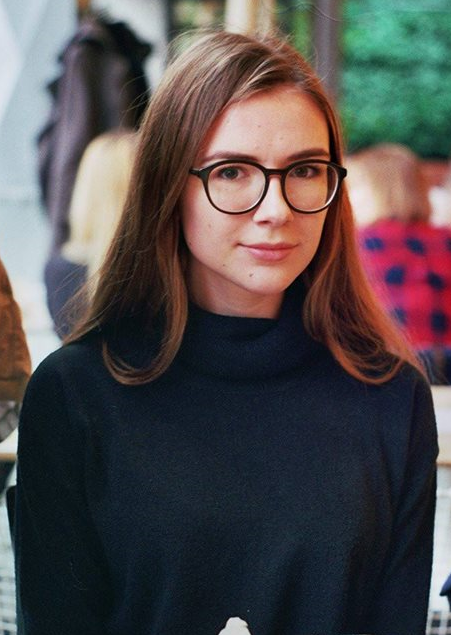
\includegraphics[width=3cm]{zdj1.png}
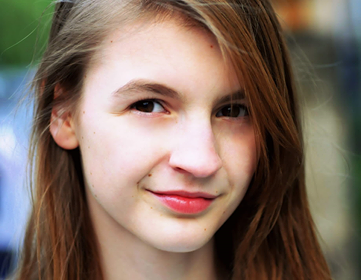
\includegraphics[width=3cm]{zdj2.png}
\end{figure}

\end{frame}

%%%%%%%%%%%%%%%%
\begin{frame}{Outline}
	\tableofcontents
\end{frame}

%%%%%%%%%%%%%%%%%%%%%%%
\section{Physics motivation}

\begin{frame}
\frametitle{Physics motivation}
The physics motivation for the measurement:
\begin{itemize}
\item a good test for the SM,
\item a measurement of inclusive and differential fiducial cross sections,
\item test of perturbative QCD calculations.
\end{itemize}

\end{frame}

\begin{frame}
\frametitle{The Feynman diagram}

\begin{figure} [H]
\centering
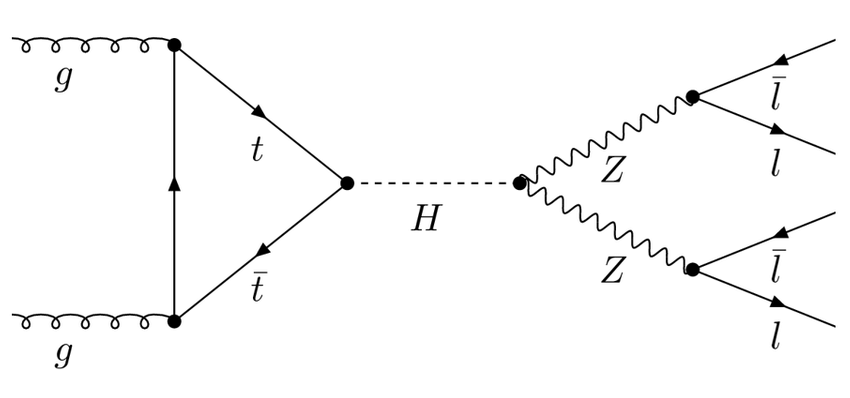
\includegraphics[width=8cm]{feynman_diagram.png}
\caption{Feynman diagram for $\hzz$ decay \cite{diagram}. }
\end{figure}

\end{frame}

%%%%%%%%%%%%%%%%%%%%%%%
\section{Event selection}

\begin{frame}
\frametitle{Event selection}
The final event-selection criteria for $ZZ^*$ production:

\begin{itemize}
\item single-electron or single-muon trigger satisfied,
\item exactly four leptons (electrons or muons) with $p_T>25, 15, 10, 7 GeV$, respectively,
\item Higgs-boson candidates are formed by selecting two $SFOS$ lepton pairs,
\item the leading pair is defined as the $SFOS$ \footnote{$SFOS$ - Same Flavour, Opposite Charge} pair with the mass $m_{\ell \ell, 1}$ closest to the $Z$ boson mass $m_Z$, and the subleading pair is defined as the SFOS pair with the mass $m_{\ell \ell, 1}$ second closest to $m_Z$ \cite{opendata}.

\end{itemize}

\end{frame}

\begin{frame}
\frametitle{Cutflow Histogram}

\begin{tabular}{cl}  
         \begin{tabular}{c}
	%\begin{figure}
           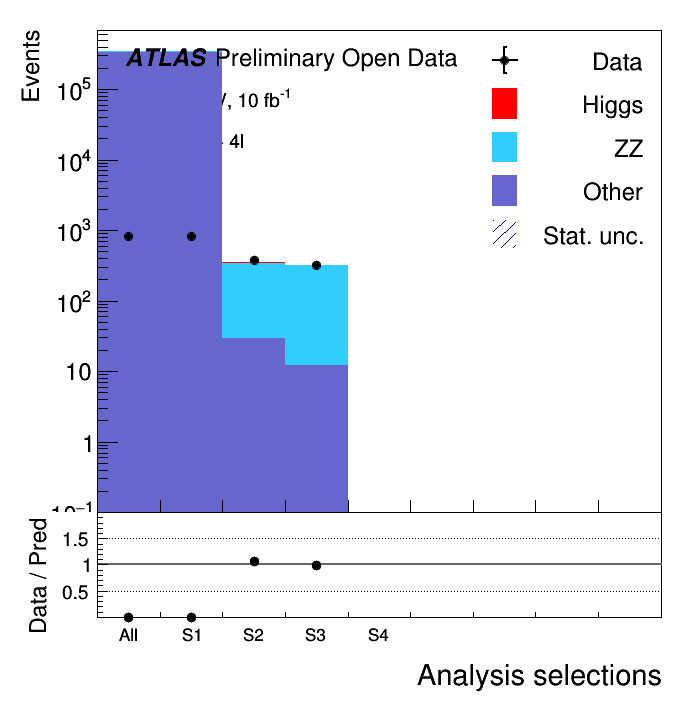
\includegraphics[width=6cm]{hist_cutflow.png}
	%\caption{The cutflow histogram.}
	%\end{figure}
           \end{tabular}
           & \begin{tabular}{l}
             \parbox{0.5\linewidth}{%  change the parbox width as appropiate
		On the cutflow histogram we can observe number of events after each selection criteria:
		\begin{itemize}
		\item $S1$ - single-electron or single-muon trigger satisfied, 
		\item $S2$ - four leptons with $p_T>25, 15, 10, 7 GeV$, 
		\item $S3$ - two SFOS lepton pairs.
		\end{itemize}

    }
         \end{tabular}  \\
\end{tabular}

\end{frame}

%%%%%%%%%%%%%%%%%%%%%%%
\section{Expected number of events}

\begin{frame}
\frametitle{Expected number of events}
Expected number of events equals:
\begin{equation}
N^{ \hzz }_{exp}=\sigma^{ \hzz }_{incl} \cdot L_{int},
\end{equation}
where:
\begin{description}
\item[$\sigma^{ \hzz }_{incl}$] = 3,62 $fb^{-1}$,
\item[$L_{int}$] = 10,06 $fb^{-1}$.
\end{description}
\vspace{1cm}
\begin{equation}
N^{\hzz}_{exp}=3.62 \: \mathrm{fb} \cdot 10.06 \: \mathrm{fb}^{-1} = 36.42.
\end{equation}

\end{frame}

%%%%%%%%%%%%%%%%%%%%%%%
\section{Background contributions}
\begin{frame}
\frametitle{Background contributions}
Processes constituting background of our analysis:
\begin{itemize}
\item non-resonant SM ZZ* production,
\item $t\bar{t}$ production,
\item Z+jets production.
\end{itemize}

\end{frame}

%%%%%%%%%%%%%%%%%%%%%%%
\section{Control plots}

%%% Number of leptons
\begin{frame}
\frametitle{Number of Leptons}

\begin{tabular}{cl}  
         \begin{tabular}{c}
           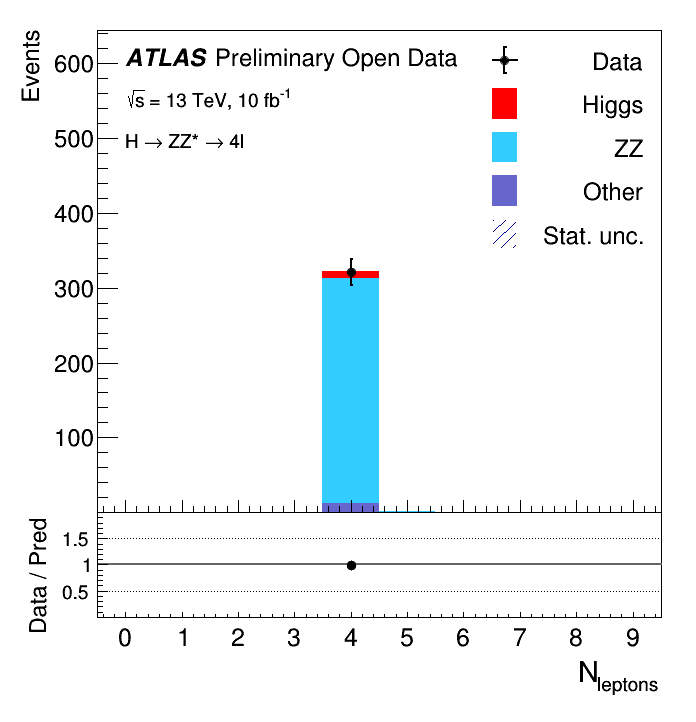
\includegraphics[width=6cm]{hist_n_leptons.png}
           \end{tabular}
           & \begin{tabular}{l}
             \parbox{0.5\linewidth}{%  change the parbox width as appropiate
	This histogram contains the number of leptons after all selection criteria.
             We can observe four leptons.
    }
         \end{tabular}  \\
\end{tabular}

\end{frame}


%%% charge
\begin{frame}
\frametitle{Charge of selected leptons}

\begin{tabular}{cl}  
         \begin{tabular}{c}
           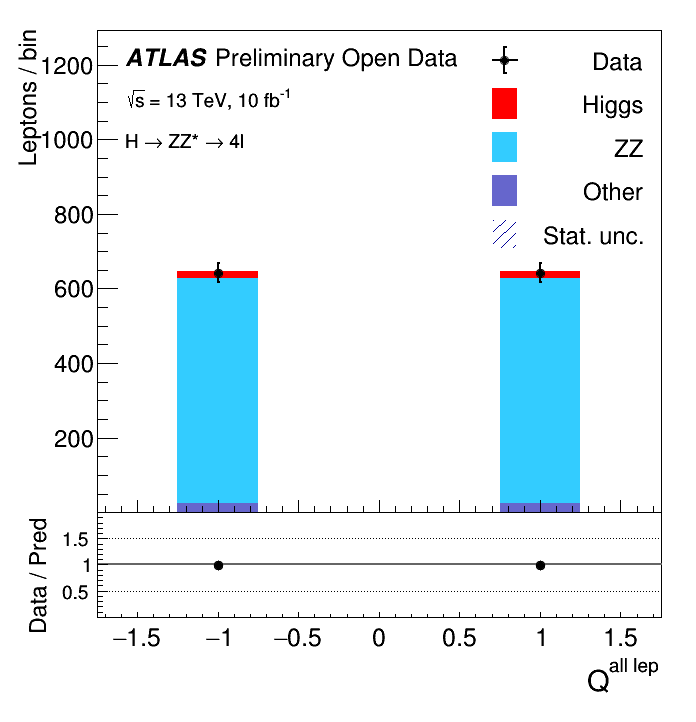
\includegraphics[width=6cm]{hist_fourleptch.png}
           \end{tabular}
           & \begin{tabular}{l}
             \parbox{0.5\linewidth}{%  change the parbox width as appropiate
		On the histogram we can observe agreement with the selection criteria. The same amount of leptions of opposite charges was selected.
    }
         \end{tabular}  \\
\end{tabular}

\end{frame}

%%% pseudorapidity, azimuthal angle, 
\begin{frame}
\frametitle{Pseudorapidity and azimuthal angle of selected leptons}

\begin{figure} [H]
\centering
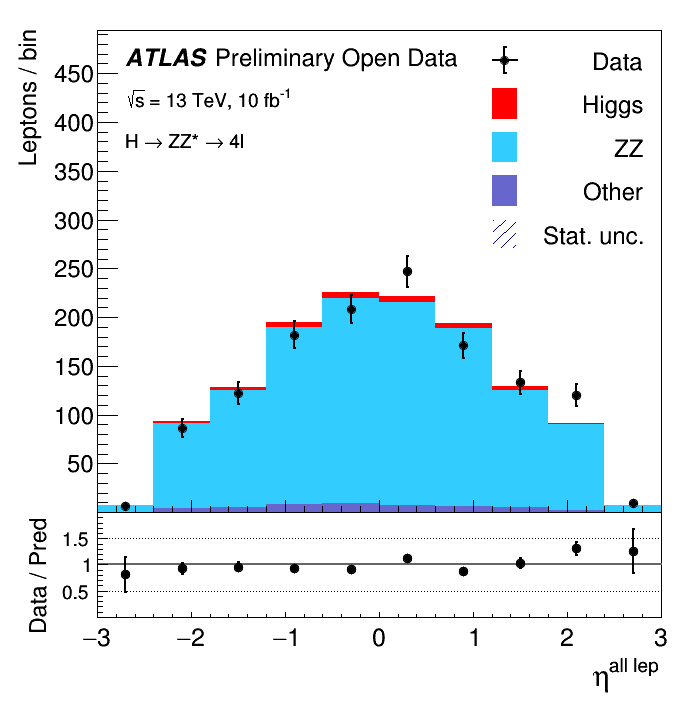
\includegraphics[width=0.4\textwidth]{hist_fourlepteta.png}
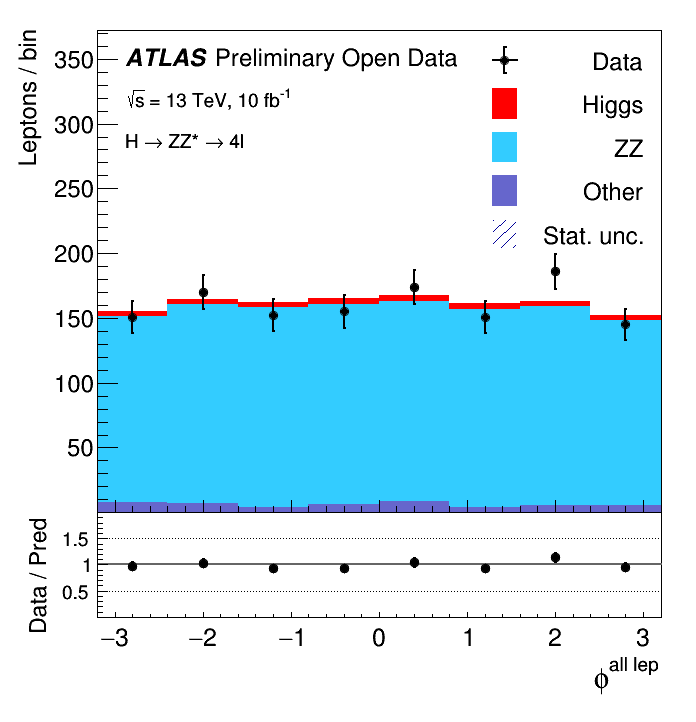
\includegraphics[width=0.4\textwidth]{hist_fourleptphi.png}
\caption{Pseudorapidity (on the left) and azimuthal angle (on the right) of selected leptons. }
\end{figure}

\end{frame}

%%% Mass of Z-boson candidates
\begin{frame}
\frametitle{Distribution of invariant masses of the reconstructed Z-boson candidates}

The histograms contains peeks for events with energy close to $90$ GeV.

\begin{figure} [H]
\centering
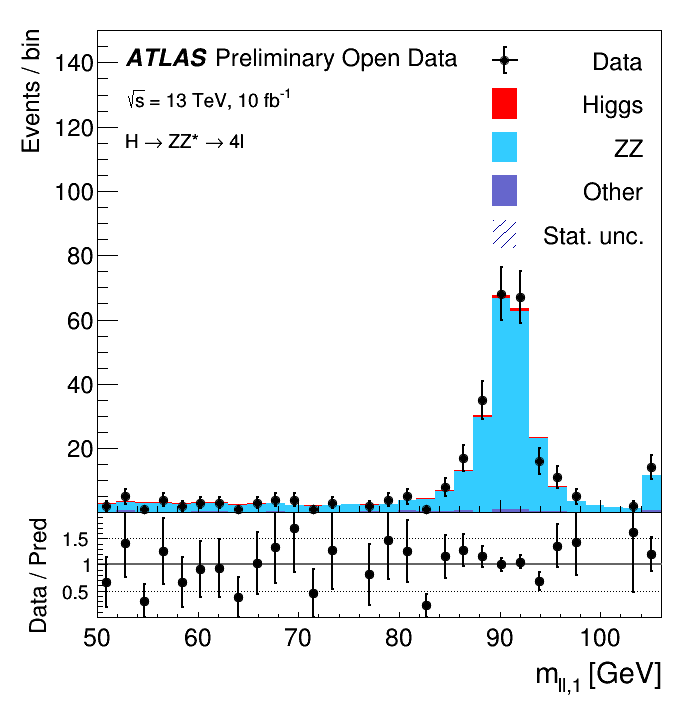
\includegraphics[width=0.4\textwidth]{hist_mLL1.png}
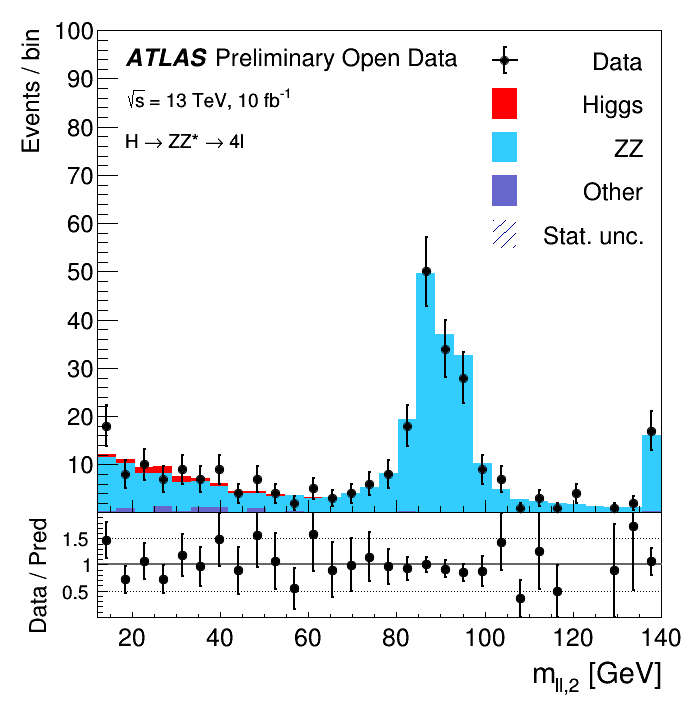
\includegraphics[width=0.4\textwidth]{hist_mLL2.png}
\caption{Distribution of invariant masses of leading and subleading SFOS pair. }
\end{figure}

\end{frame}

%%% 4 lepton mass
\begin{frame}
\frametitle{Four-lepton mass distribution of selected events}

On both histogram we can observe two peeks, one with $m_{4l} = 90 $ GeV and other, the Higgs boson candidate with $m_{4l} = 125 $ GeV.

\begin{figure} [H]
\centering
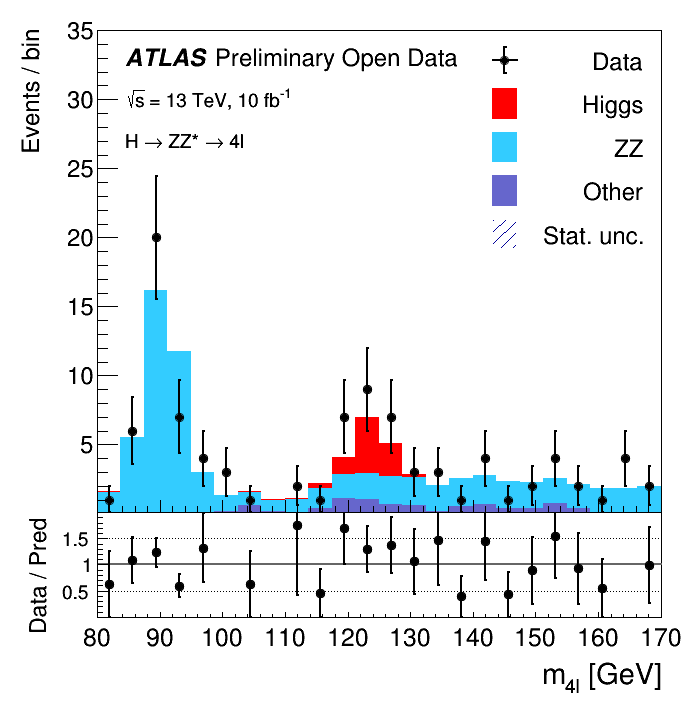
\includegraphics[width=0.4\textwidth]{mass_four_lep.png}
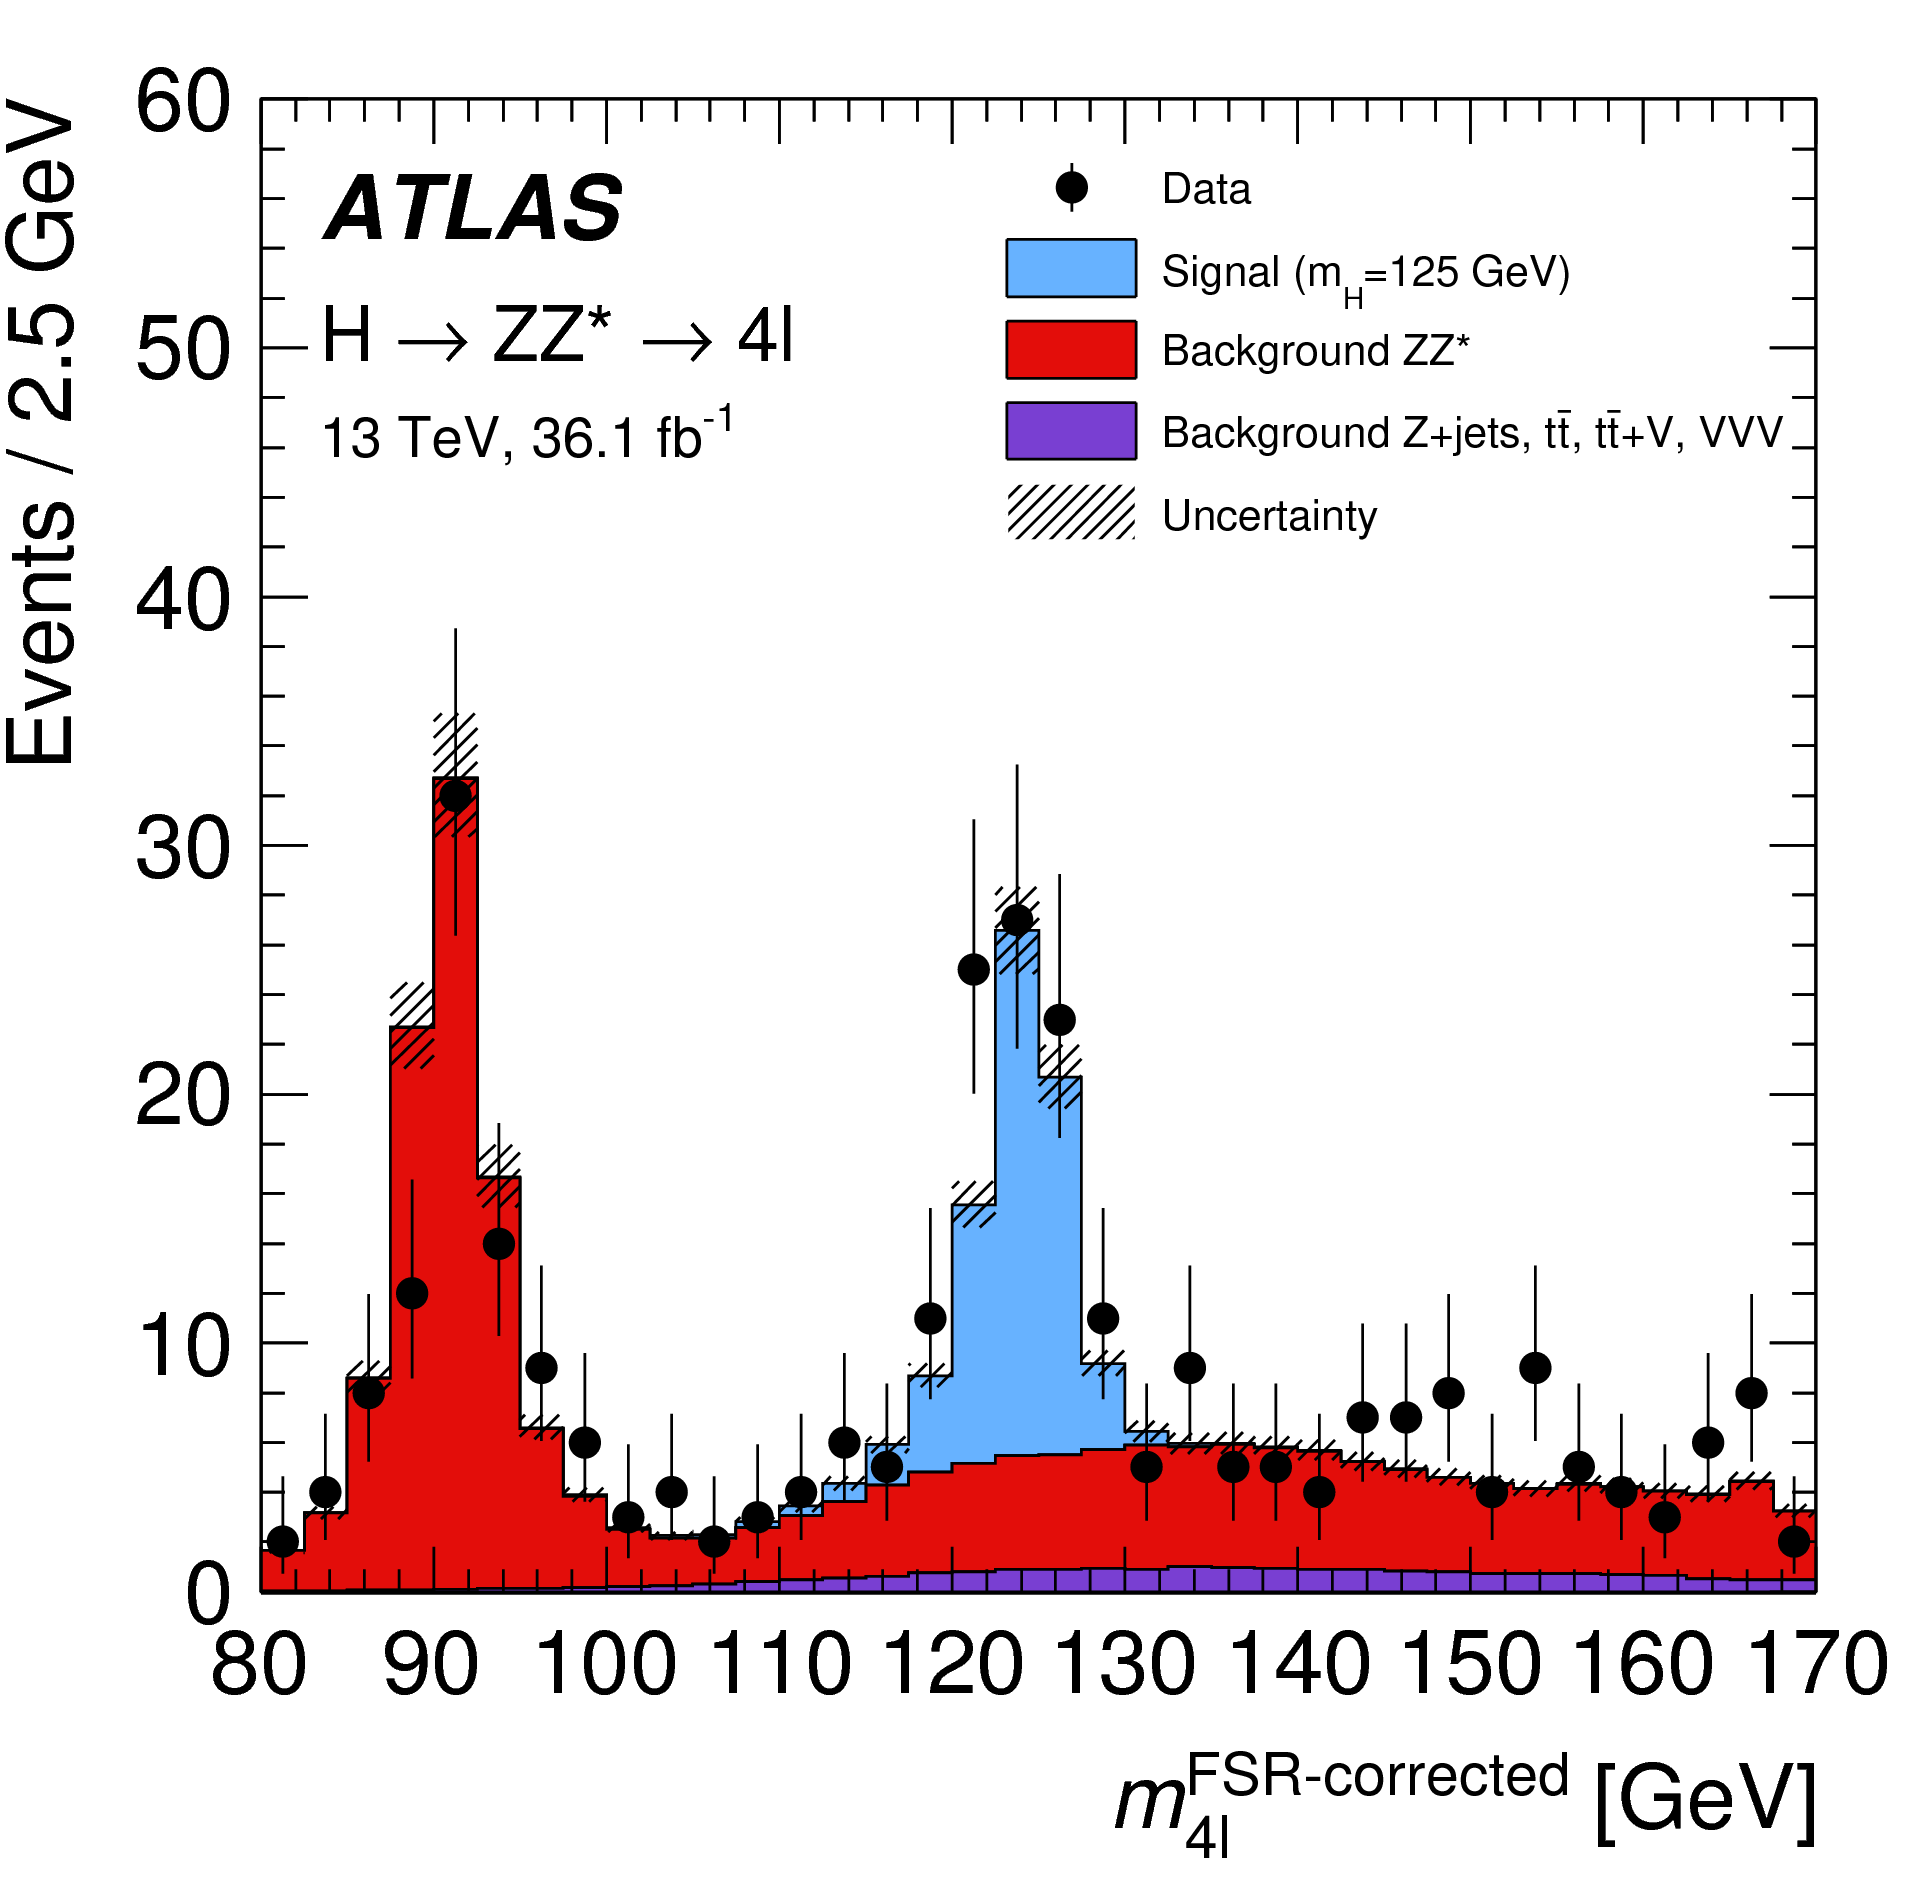
\includegraphics[width=0.4\textwidth]{mass_four_lep_pub.png}
\caption{ Distribution of four-lepton mass extreacted from our analysis (on the left) and the ATLAS publication (on the right) \cite{hzz}. The ATLAS' histogram is corrected for final-state radiation.}
\end{figure}

\end{frame}

%%% traverse momentum - comparison
\begin{frame}
\frametitle{Traverse momentum of the four leptons}


\begin{figure} [H]
\centering
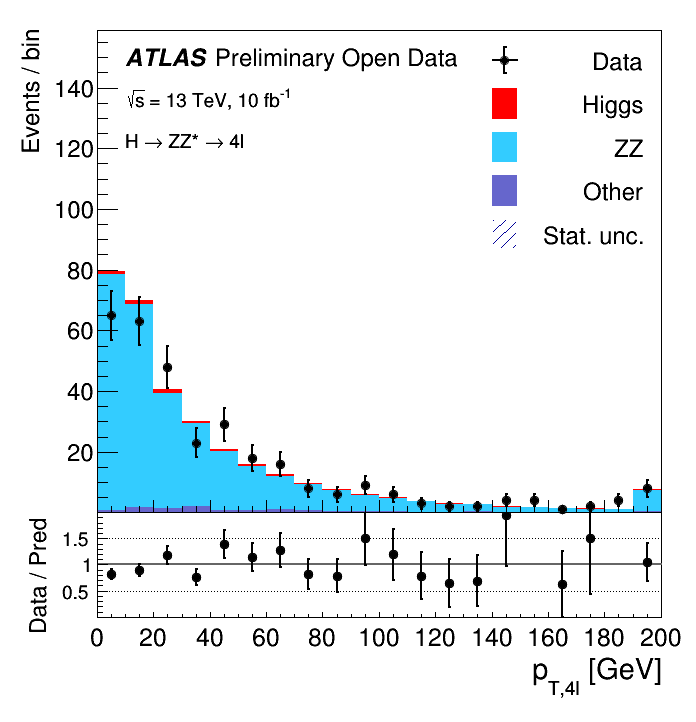
\includegraphics[width=0.4\textwidth]{hist_fourlepsys_pt.png}
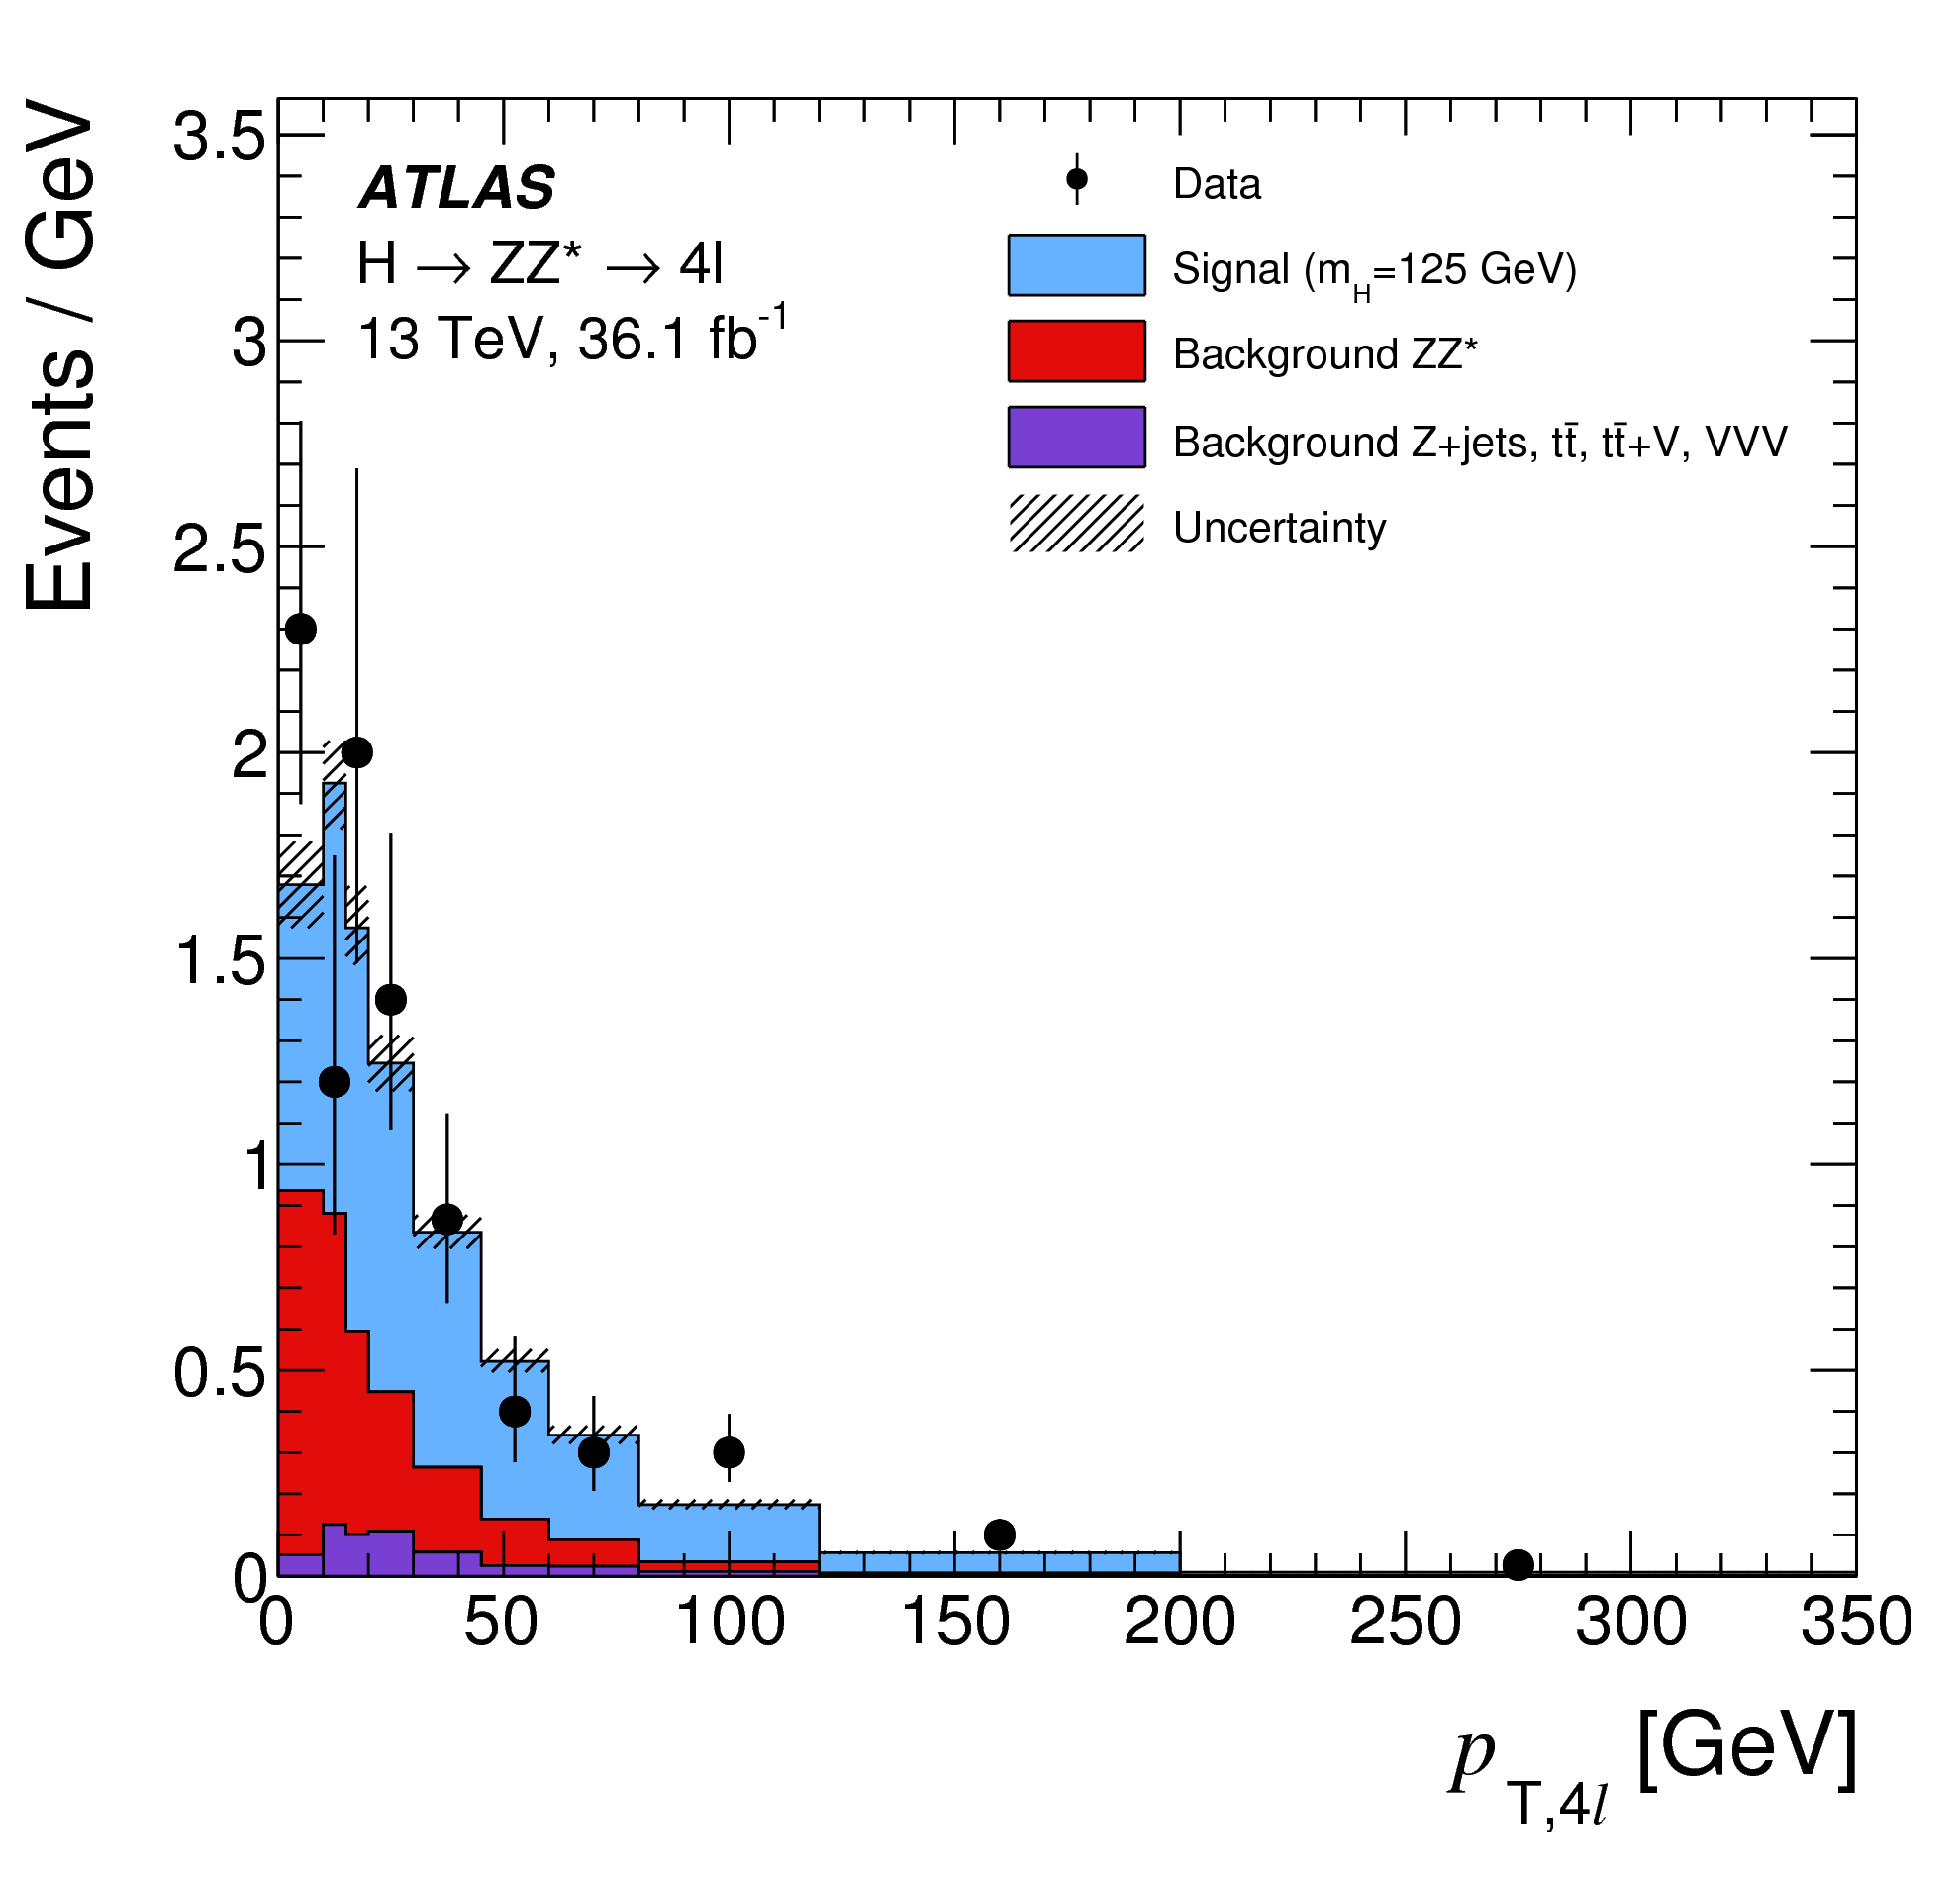
\includegraphics[width=0.4\textwidth]{hist_fourlepsys_pt_pub.png}
\caption{ Distribution of traverse momentum for selected events extracted from out analysis (left) and the ATLAS publication (right) \cite{hzz}. The background ZZ contribution in right histogram is much smaller.}
\end{figure}

\end{frame}

%%% jet multiplicity - comparison
\begin{frame}
\frametitle{Jet multiplicity}

\begin{figure} [H]
\centering
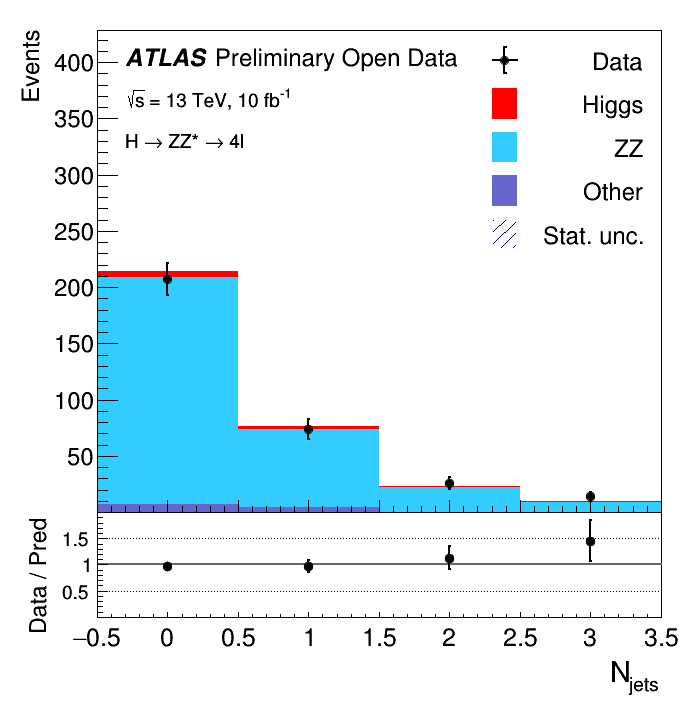
\includegraphics[width=0.4\textwidth]{hist_n_jets.png}
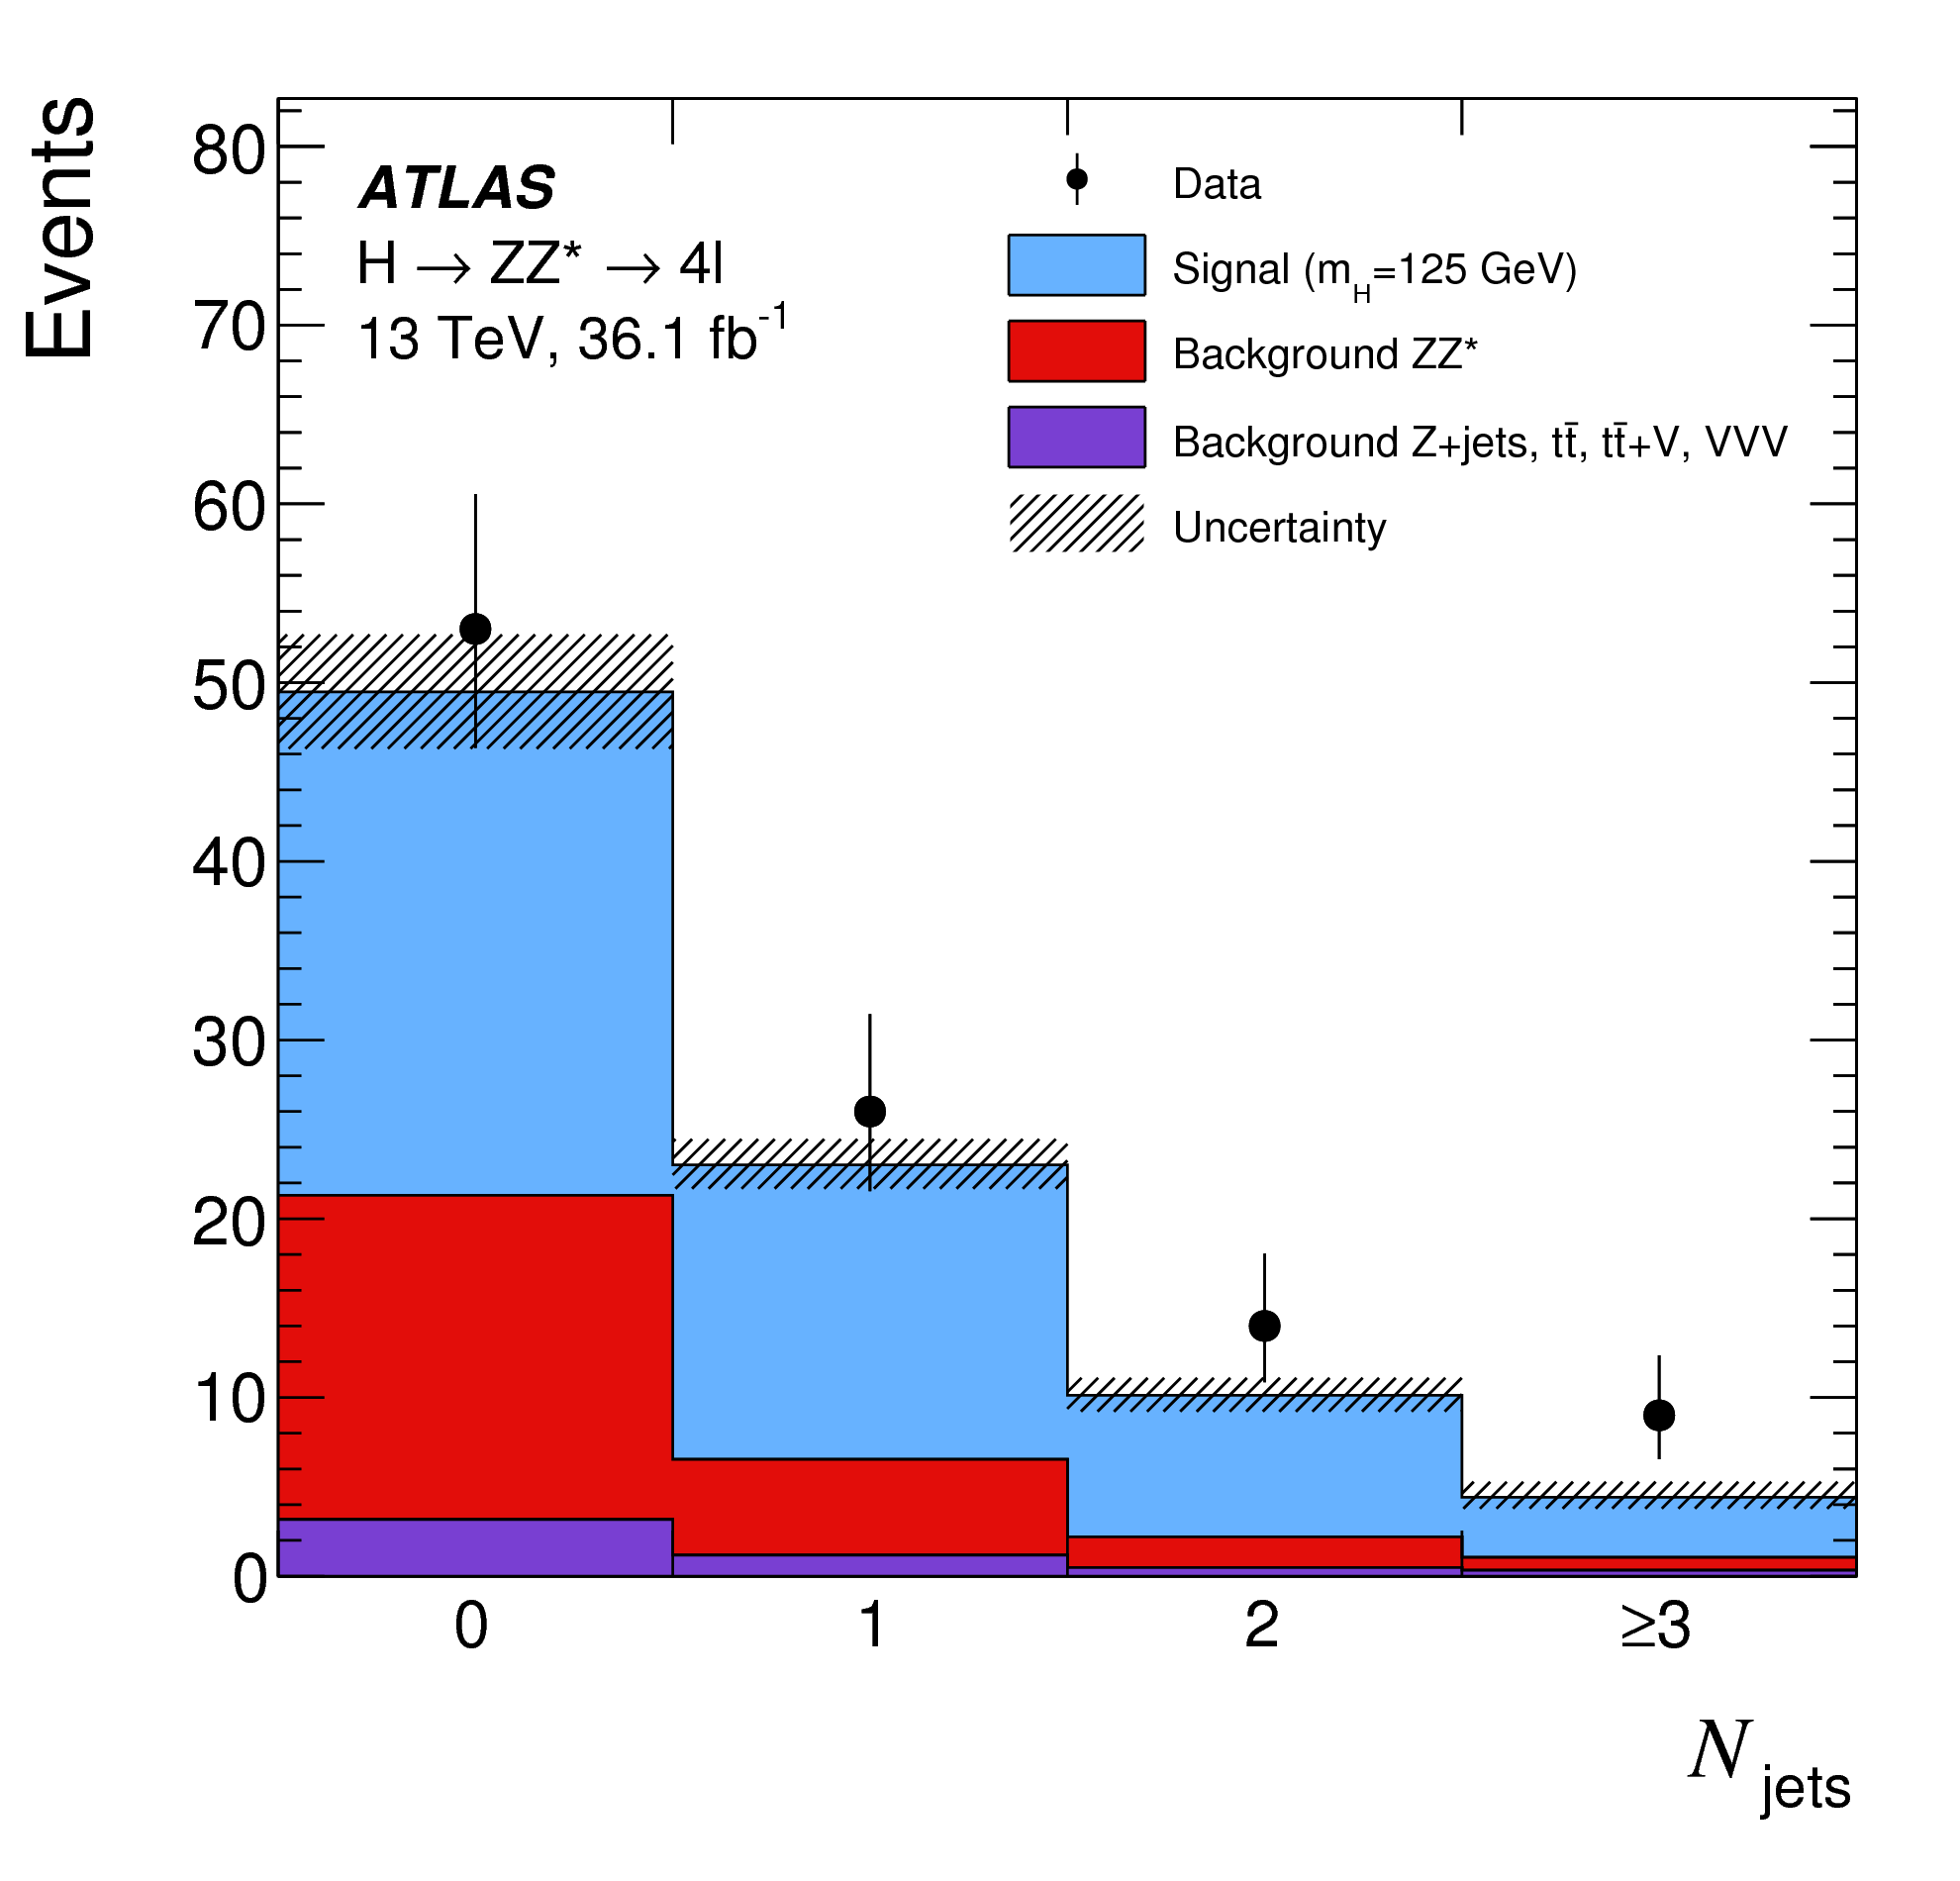
\includegraphics[width=0.4\textwidth]{hist_n_jets_pub.png}
\caption{ Jet multiplicity in selected events extracted from out analysis (left) and the ATLAS publication (right) \cite{hzz}. The background ZZ contribution in right histogram is much smaller.}
\end{figure}

\end{frame}


%%%%%%%%%%%%%%%%%%%%%%%
\section{Cross-section measurement}

%% C-factor calculations
\begin{frame}
In our analysis, there were \textbf{four} correction factors:
\begin{eqnarray}
C_1=C_{4\mu}=0.64 \pm 0.04 \nonumber \\
C_2=C_{2e2\mu}=0.55 \pm 0.03 \nonumber \\
C_3=C_{2\mu2e}=0.48 \pm 0.05 \nonumber \\
C_4=C_{4e}=0.43 \pm 0.06 \nonumber \\
\end{eqnarray}
\vspace{1cm}
We took a "simplified approach" and used $C=\frac{1}{4}\sum_{i=1}^{4} C_i=\textbf{0.53}$
\end{frame}

%%% Cross-section measurement calc
\begin{frame}
\frametitle{Cross-section measurement}
Cross-section of $\hzz$ was calculated using the following formula:
\begin{equation}
\sigma^{\hzz}=\frac{N_{data}-N_{bkg}}{C\cdot L_{int}}=\frac{N_{obs}}{C\cdot L_{int}} ,
\end{equation}
where:
\begin{description}
\item[$N_{data}$] - number of all events in data; $N_{data}=321$,
\item[$N_{bkg}$] - nubmer of background events; $N_{bkg}=315$,
\item[$N_{obs}$] - number of observed $\hzz$; $N_{obs}=6$,
\item[$C$] - correction factor; $C=0.525$,
\item[$L_{int}$] - integrated luminosity; $L_{int}=10.06 \: \mathrm{fb}^{-1}$.
\end{description}
\vspace{1cm}
\begin{equation}
\sigma^{\hzz}=\frac{321-315}{0.525\cdot 10.06}=\frac{6}{0.525\cdot 10.06}=1.14 \: [\mathrm{fb}]
\end{equation}

\end{frame}

%%% Systematic uncertainties for data
\begin{frame}
\frametitle{Systematic uncertainties for data}

\begin{figure} [H]
\centering
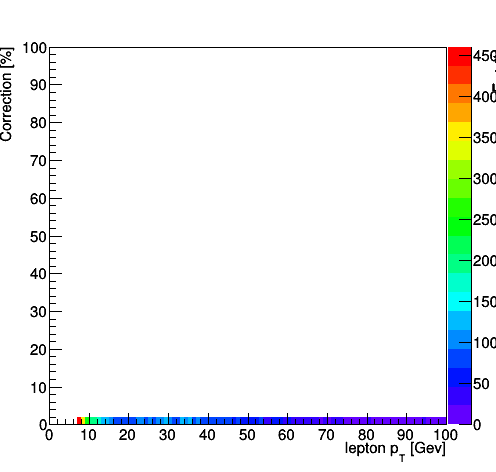
\includegraphics[width=0.5\textwidth]{syst1_data.png}
\caption{The histogram shows a size of correction in percentages for the data in the analysis. }
\end{figure}

\end{frame}

%%% Systematic uncertainties for signal
\begin{frame}
\frametitle{Systematic uncertainties for signal}

\begin{figure} [H]
\centering
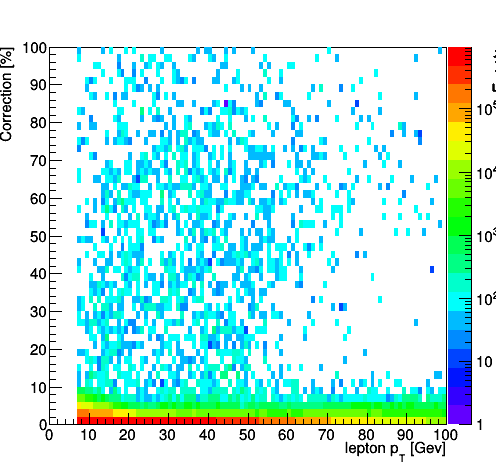
\includegraphics[width=0.5\textwidth]{syst1_signal.png}\hfill
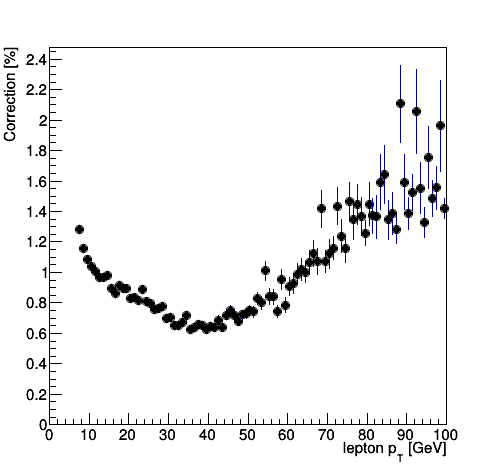
\includegraphics[width=0.5\textwidth]{syst2_signal.png}
\caption{The histogram shows a size of correction in percentages for the MC data in the analysis. The correction is below $2.5\%$. }
\end{figure}

\end{frame}

%%% Systematic uncertainties calc
\begin{frame}
\frametitle{Systematic uncertainties}
The cross-section measurement was repeated with correction on leptons' traverse momentums.\\
\vspace{0.5cm}

Case 1: The systematic uncertainties were added to the leptons' traverse momentums.
\textbf{Four} events were observed.
\begin{equation}
\delta_{syst, 1} = \sigma^{\hzz} - \sigma^1 = | 1.136 - 0.757 | = 0.379 \: [\mathrm{fb}]
\end{equation}

Case 2: The systematic uncertainties were subracted from the leptons' traverse momentums.
\textbf{Eleven} events were observed.
\begin{equation}
\delta_{syst, 2} = \sigma^{\hzz} - \sigma^2 = | 1.136 - 2.083 | = 0.946 \: [\mathrm{fb}]
\end{equation}

As the final systematic uncertainty of the cross section measurement maximum value of $\delta_{syst, 1}, \delta_{syst, 2}$ was taken.

\begin{equation}
\delta_{syst_A} = 0.946 \: [\mathrm{fb}]
\end{equation}

\end{frame}

%%% Statistical, systematic and luminosity uncertainties of cs
\begin{frame}
\frametitle{Statistical, systematic and luminosity uncertainties of cross-section}
Error propagation rule was used in cross-section's uncertainty calculations:
\begin{equation}
\delta_{\sigma}=\sqrt{\sum_i\qty(\grande \pdv{\sigma}{x_i}\cdot \delta_{x_i} )^2} = \sqrt{\qty(\grande \frac{1}{C\cdot L_{int}}\cdot \delta_{N_{data}})^2 + \qty(\grande \frac{-N_{obs}}{C\cdot L_{int}^2}\cdot \delta_{L_{int}})^2 + \qty(\grande \frac{-N_{obs}}{C^2\cdot L_{int}}\cdot \delta_{C})^2 } ,
\end{equation}
where:
\begin{description}
\item[$\delta_{N_{data}}$] = $\sqrt{N_{data}}=17.92$,
\item[$\delta_{L_{int}}$] = $0.37 \: \mathrm{fb}^{-1}$,
\item[$\delta_C$] = $\max(\abs{C_i-C})=0.12, \; i=1, 2, 3, 4$.
\end{description}
\vspace{1cm}
Based on the formula above, all required uncertainties were calculated:
\begin{eqnarray}
    \delta_{stat}=3.40 \nonumber \\
    \delta_{syst}=\sqrt{\delta_{syst_A}^2 +\delta_{syst_A}^2}=0.98 \nonumber \\
    \delta_{lumi}=0.05 \nonumber
\end{eqnarray}
\vspace{1cm}
Eventually, cross-section value can be expressed as: $\sigma^{\hzz, \: \mathrm{nom}}=\textbf{1.14} \: \pm 3.4 \: \mathrm{(stat)} \: \pm 0.98 \: \mathrm{(syst)} \: \pm 0.05 \: \mathrm{(lumi) \: fb}$

\end{frame}

%%%%%%%%%%%%%%%%%%%%%%%
\section{Ideas for possible measurements}

%%%%%%%%%%%%%%%%%%%%%%%
\section{Bibliography}
%%%%%%%%%%%%%%%%%%%%%%%
\begin{frame}[allowframebreaks]{Bibliography}
\begin{thebibliography}{9}
		\setbeamertemplate{bibliography item}[article]
		\bibitem{opendata}
			{The ATLAS collaboration\newblock Review of the 13 TeV ATLAS Open Data release \newblock \url{https://cds.cern.ch/record/2707171}}
		\bibitem{hzz}
			{Aaboud, Morad and others \newblock Measurement of inclusive and differential cross sections in the $ \hzz $ decay channel in pp collisions at $s√ = 13 TeV$ with the ATLAS detector \newblock \url{http://dx.doi.org/10.1007/JHEP10(2017)132}}
		\bibitem{diagram}
			{Passon, Oliver \newblock On the interpretation of Feynman diagrams, or, did the LHC experiments observe the Higgs to gamma gamma decay?}
\end{thebibliography}
\end{frame}
\end{document}
